\begin{chapter}{Testes e Resultados}
\vspace{-0.5cm}
Neste capítulo é mostrado o perfil dos participantes que aceitaram realizar os
testes com o protótipo desenvolvido neste trabalho, bem como o ambiente onde os
testes ocorreram e as tarefas elaboradas para serem realizadas pelos
participantes.  Por último são apresentados os resultados quantitativos e
qualitativos do teste.  %ok 

\vspace{-0.5cm}
\begin{section}{Participantes}

O estudo foi realizado com 7 pessoas do sexo masculino e 3 pessoas do sexo
feminino, totalizando 10 participantes, com idades entre 21 e 28 anos.
Todos os participantes são estudantes de graduação ou pós-graduação da
Universidade Federal do pará (UFPA). O único critério exigido para participar
dos testes era que o participante deveria ter uma certa familiaridade com os
\textit{websites} utilizados nas tarefas.  

A seleção dos voluntários ocorreu através de uma breve conversa com o
participante do experimento, convidando-o a realizar o teste aplicado neste
trabalho. Após a aceitação do participante, o trabalho desenvolvido foi então
apresentado verbalmente, demonstrando a motivação do estudo, todos os objetivos,
a estimativa do tempo de duração do teste e as etapas de cada tarefa que
seria realizada. 

Logo após a apresentação do trabalho, o voluntário deveria ler o TCLE (Termo de
Consentimento Livre e Esclarecido), onde foi estabelecido que, ao assinar o
termo, o participante declarava estar ciente de que os dados coletados nos
testes seriam utilizados unicamente para fins de pesquisa acadêmica. Este termo
deixa claro o objetivo do trabalho, informando alguns pontos sobre a restrição
dos dados do participante e declarando por fim que o participante aceitaria os
termos. Após assinar o TCLE, o voluntário estava habilitado a realizar as
tarefas elaboradas. 

\end{section}

\begin{section}{Ambientes de Testes e Procedimentos}

O ambiente onde os testes foram realizados é mostrado na
Figura~\ref{fig:ambiente}.  Como pode ser visto, uma \textit{webcam} foi
posicionada em frente do usuário para capturar os \textit{frames} em tempo real
de seu rosto. O dispositivo de sopro desenvolvido foi fixado próximo a boca do
usuário graças a um \textit{headset} modificado que serviu como suporte de
sustentação que, independentemente da posição da cabeça do usuário, sempre
mantinha o dispositivo de sopro em frente à sua boca.

\begin{figure}[!h]
	\centering
	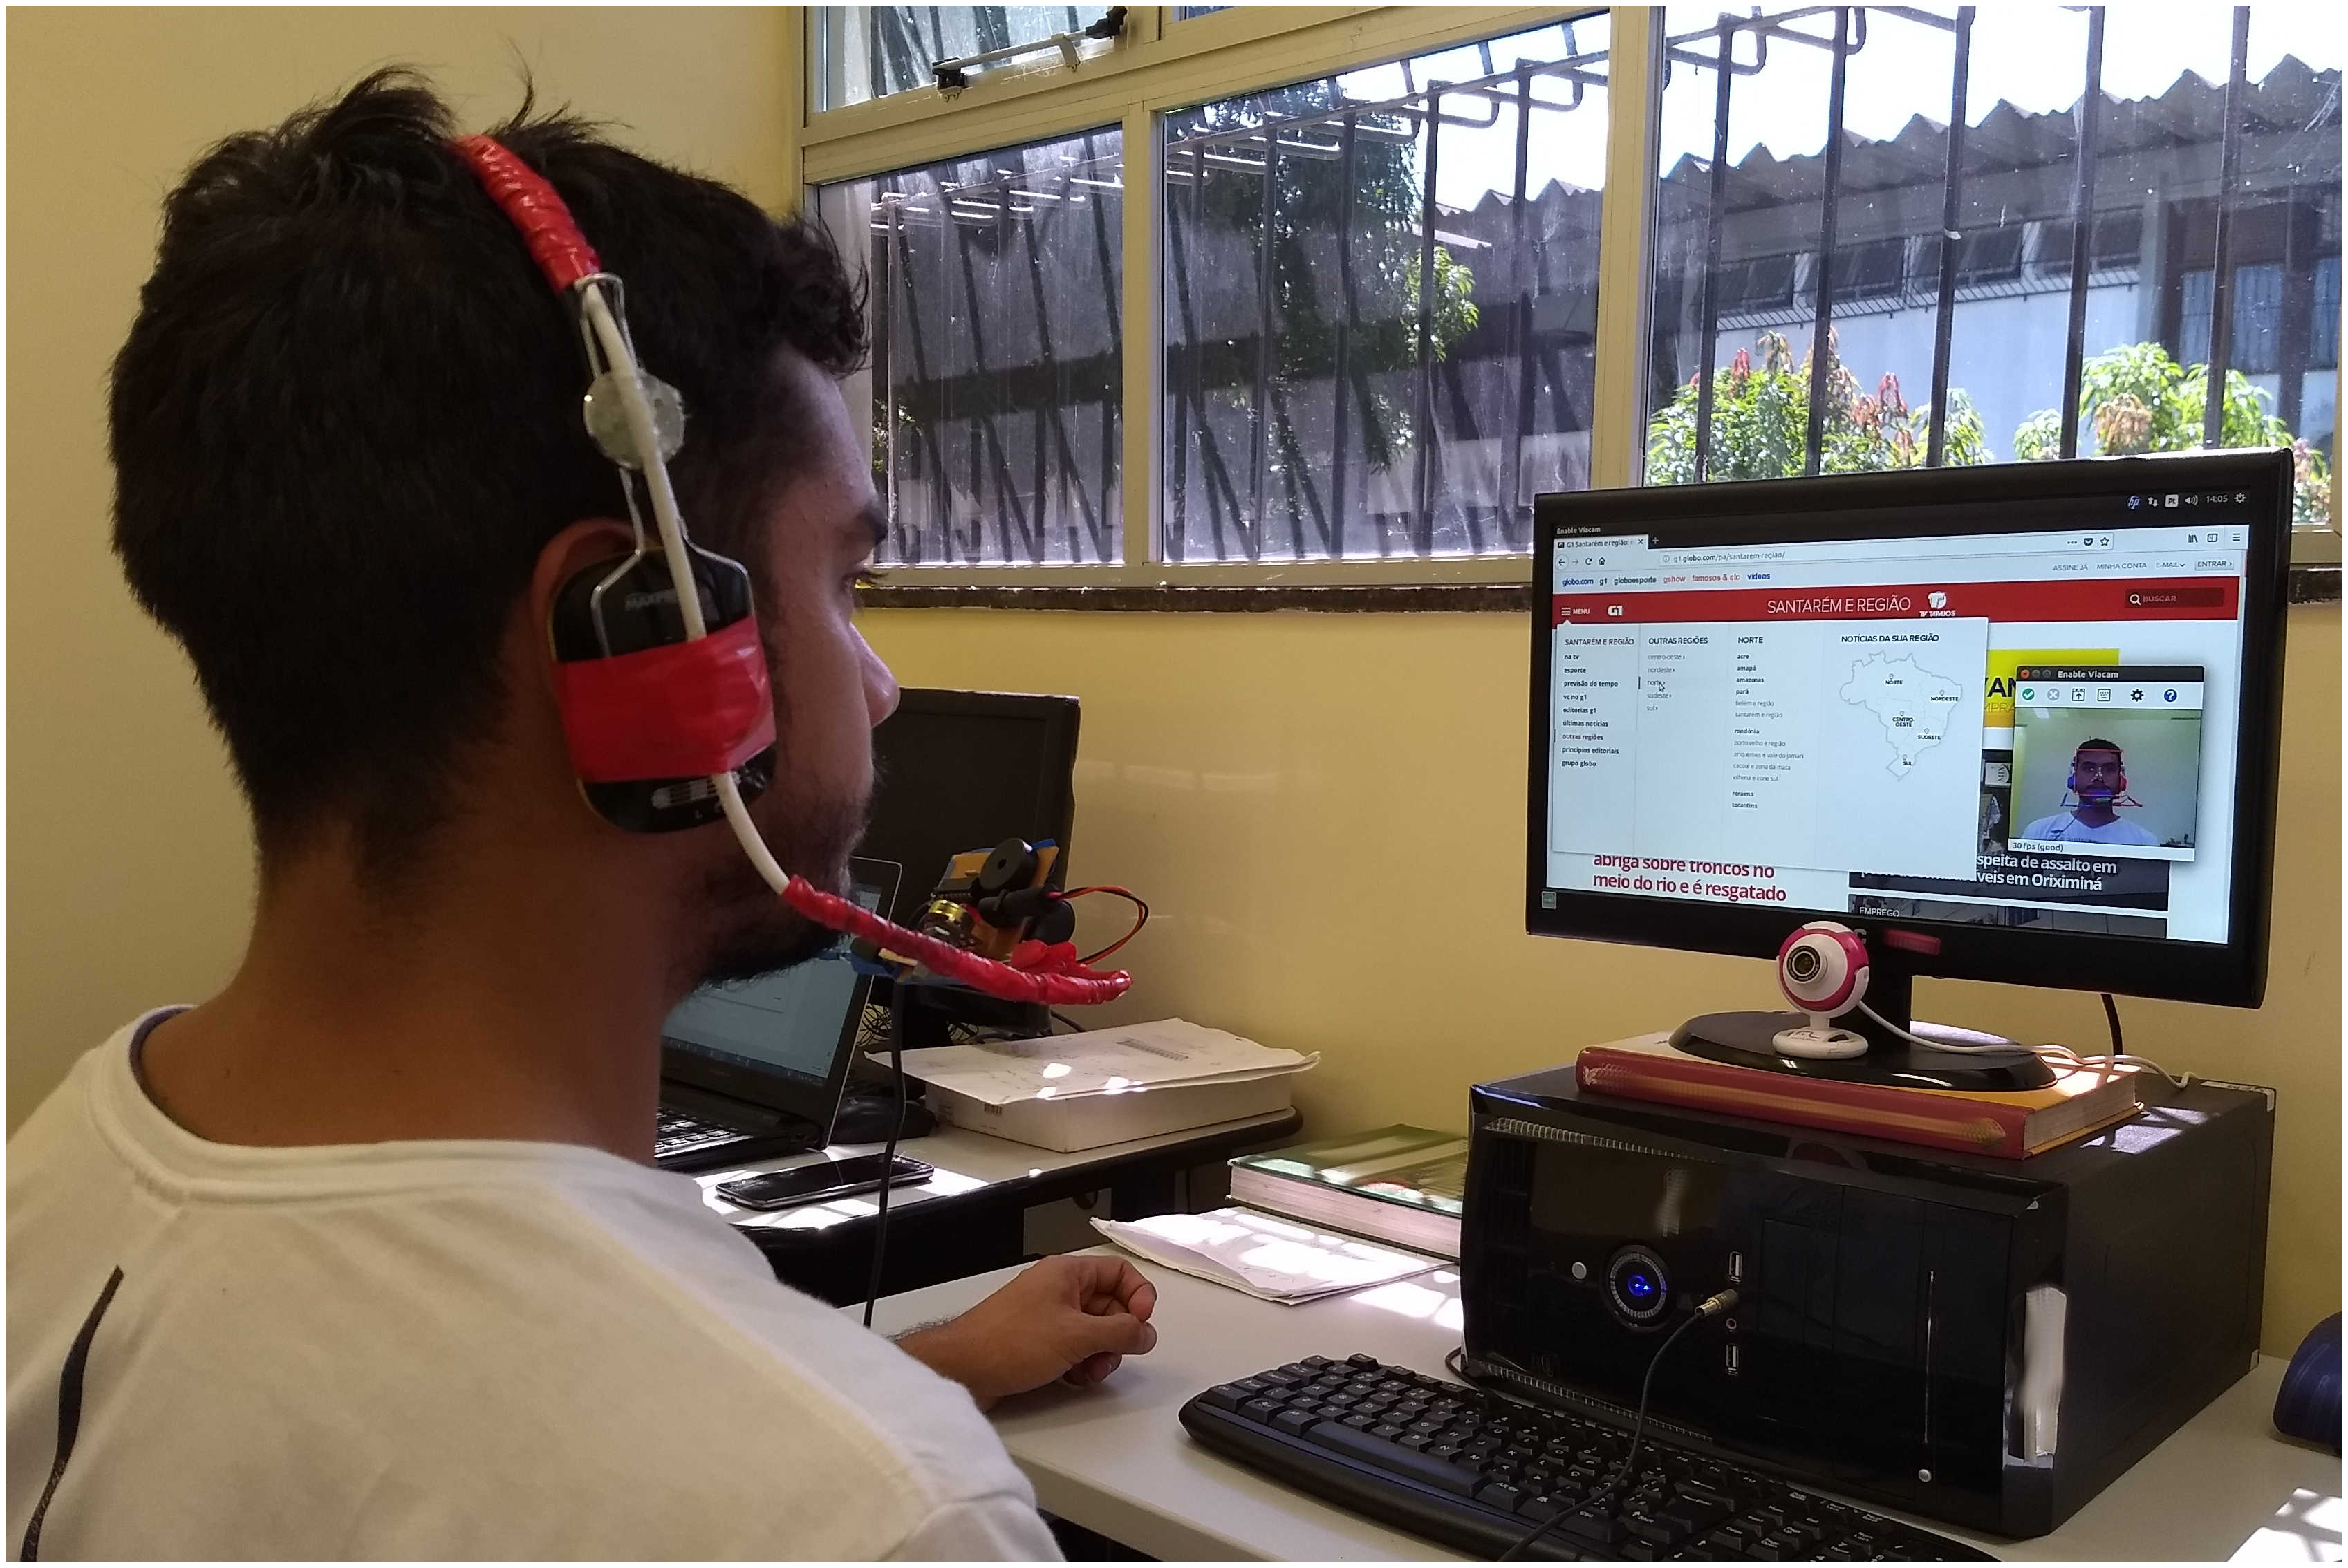
\includegraphics[width=0.95\linewidth]{fig/denes}
	\caption{Um usuário realizando as tarefas no ambiente de teste.}
	\vspace{-1cm}
	\caption*{\textbf{Fonte: }Elaborada pelo autor.}
	\label{fig:ambiente}
\vspace{-0.5cm} 
\end{figure}

Os testes foram realizados individualmente com todos os participante durante a
luz do dia. Todos estavam devidamente acomodados em uma cadeira com apoio para
a costa. O ambiente estava totalmente iluminado com a luz do sol e também com 
lâmpadas fluorescentes. Os participantes foram questionados se estariam
sentido algum desconforto  no ambiente de teste e todos relataram que
estavam confortáveis. 

O computador utilizado possui um processador Intel Core i5 da 4ª geração,
memória RAM de 4~GB e 1~TB de espaço de armazenamento com o sistema operacional
Ubuntu 16.04 Xenial Xerus x64. O monitor é um AOC E1670SWU de LED com 15,6
polegadas e com resolução de 1366 $\times$ 768.

\begin{figure}[!b]
	\centering
	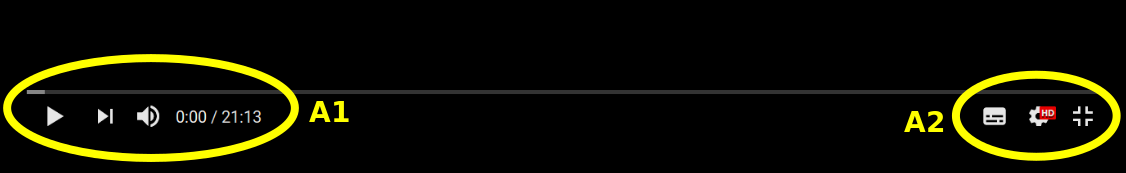
\includegraphics[width=.9\linewidth]{fig/YT}
	\caption{Áreas de interesse do \textit{website} YouTube.}
	\vspace{-1cm}
	\caption*{\textbf{Fonte: }Elaborada pelo autor.}
	\label{fig:youtube}
\end{figure}

\begin{figure}[!b]
	\centering
	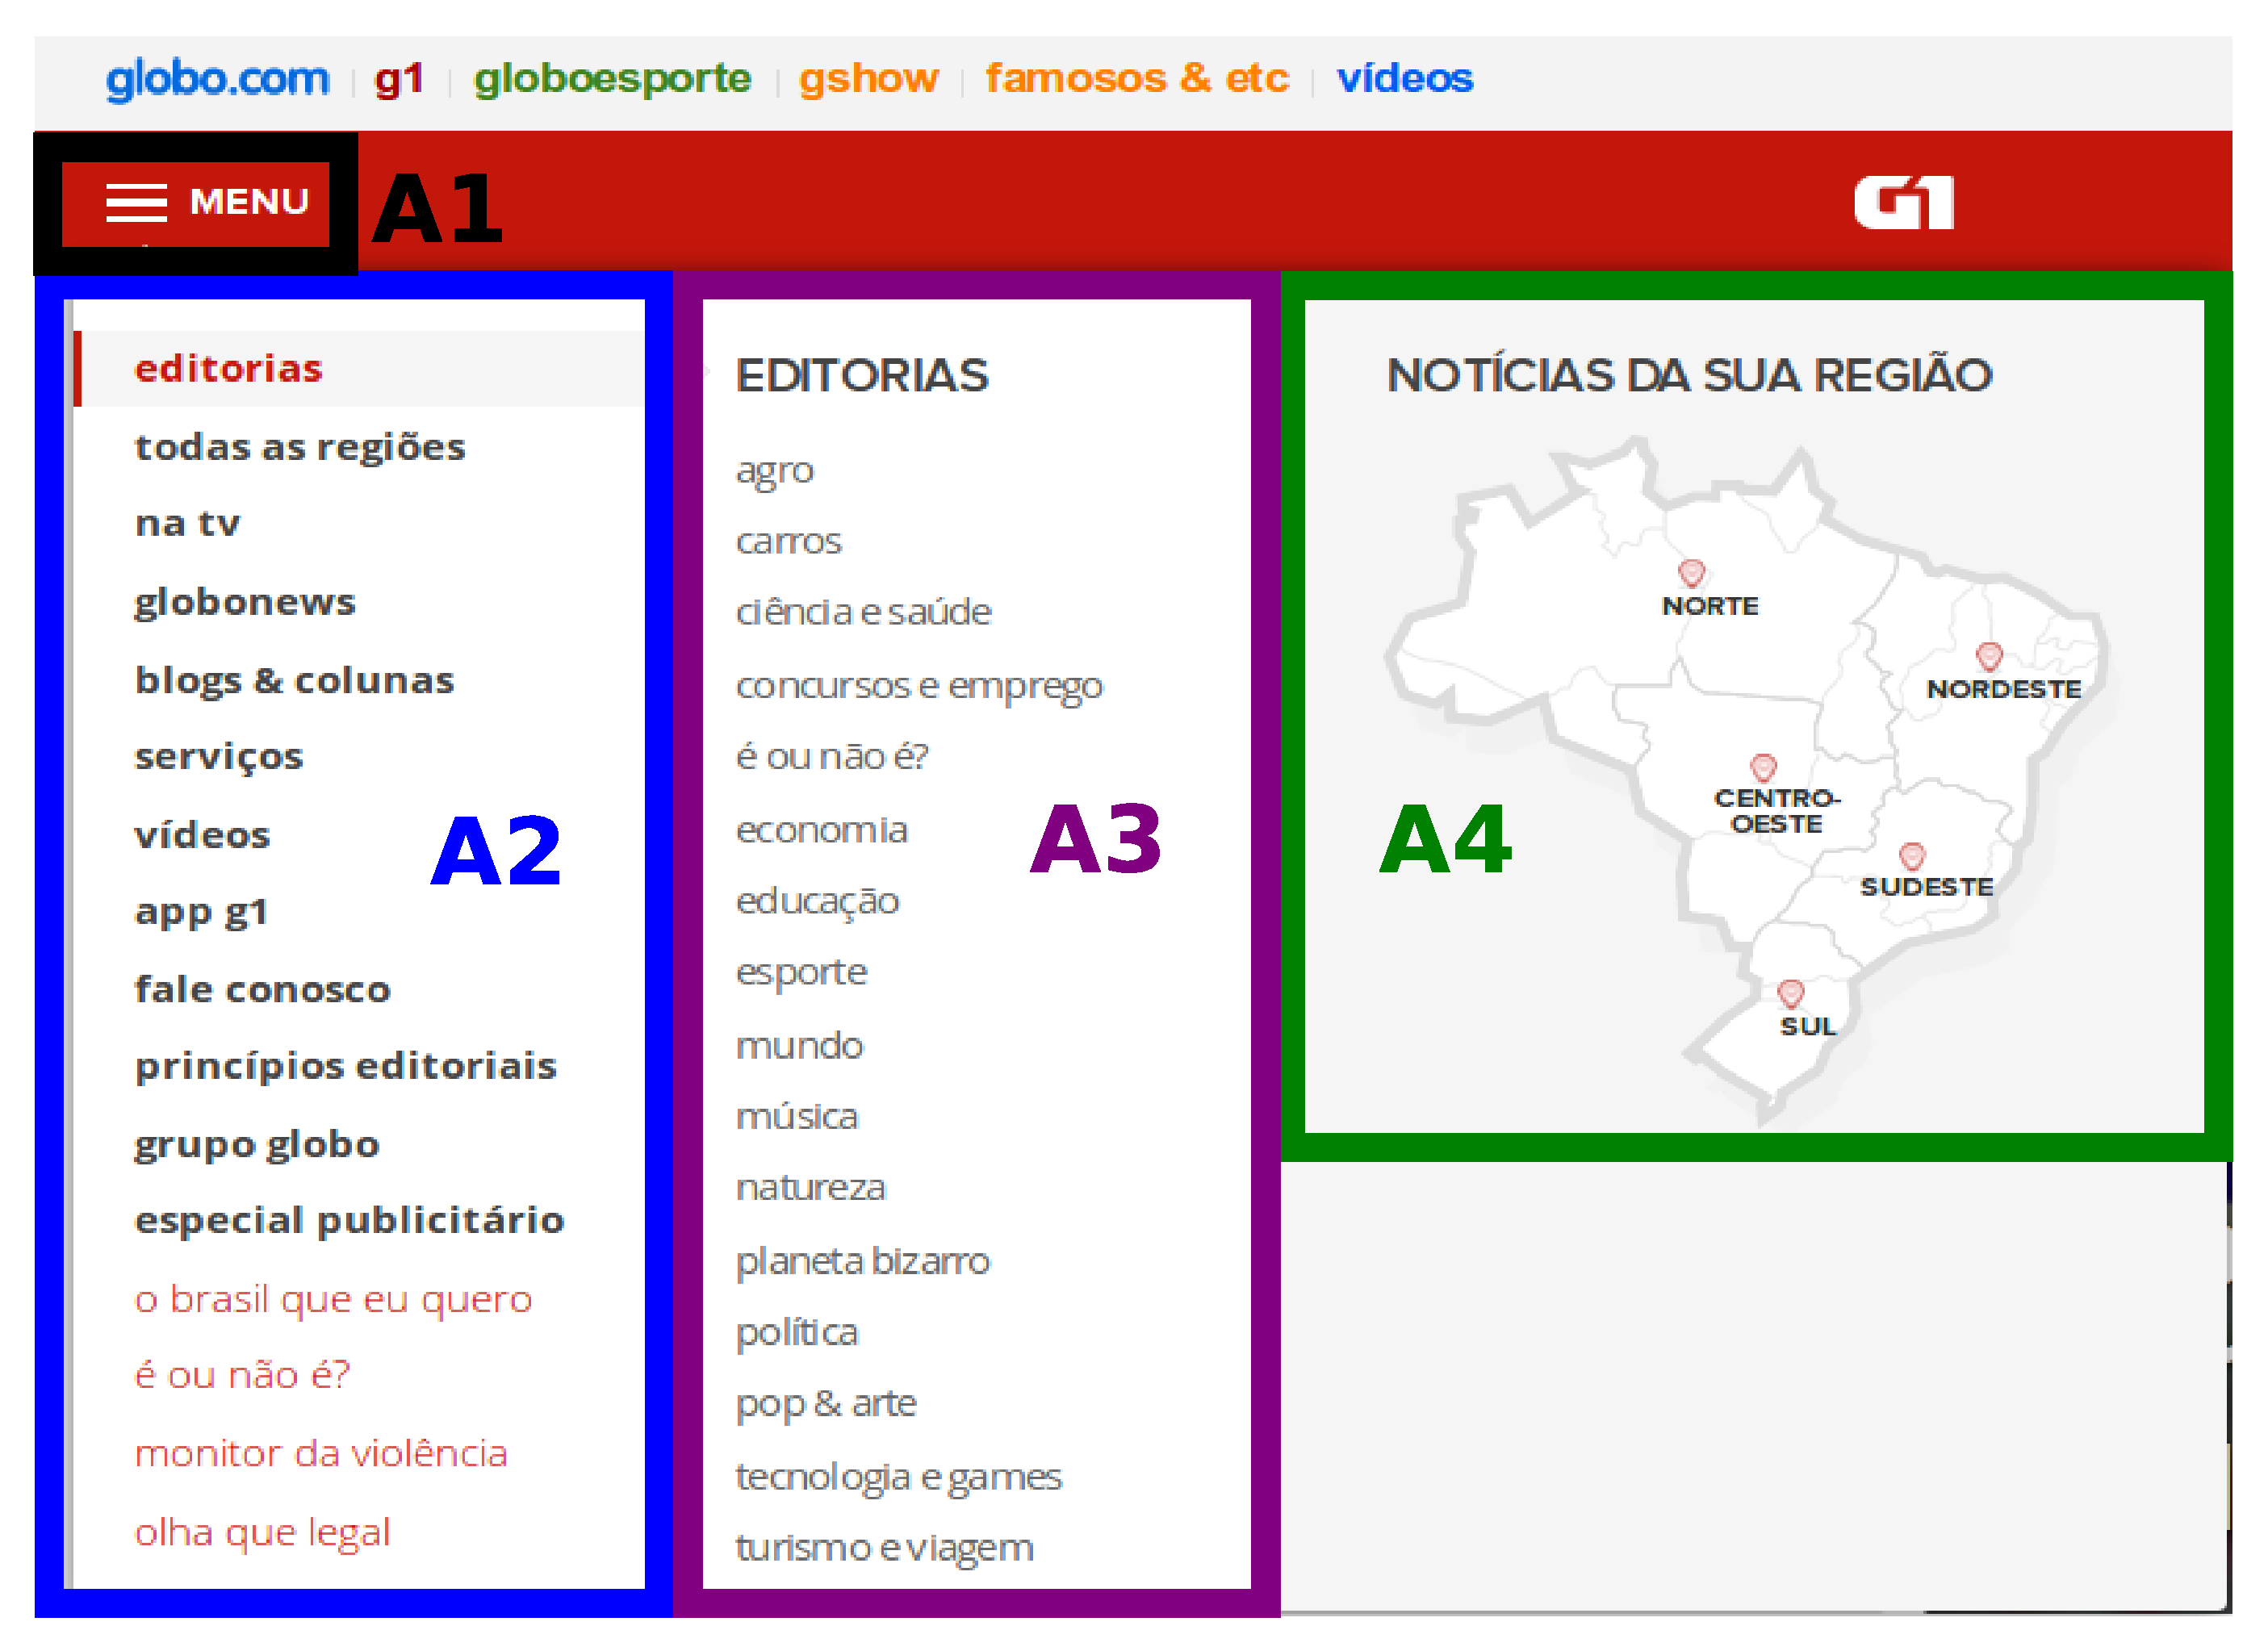
\includegraphics[width=.9\linewidth]{fig/g1}
	\caption{Áreas de interesse do \textit{website} G1.}
	\vspace{-1cm}
	\caption*{\textbf{Fonte: }Elaborada pelo autor.}
	\label{fig:g1}
\end{figure}

As tarefas dos testes foram realizadas nos \textit{websites}
YouTube (\url{https://www.youtube.com/}) e
G1 (\url{https://g1.globo.com/}), mostrados nas
Figuras~\ref{fig:youtube} e~\ref{fig:g1}, respectivamente, com suas respectivas
áreas de interesse destacados em retângulos coloridos e rotulados como A1, A2,
etc. Os \textit{websites} foram escolhidos por não serem totalmente adaptados
para tecnologias alternativas que facilitam a navegação para pessoas com
deficiência. Quando é utilizado o \textit{dwell time} como método de clique, por
exemplo, assistir um vídeo no modo de tela cheia no YouTube torna-se um desafio,
pois o usuário é forçado a mover o cursor do \textit{mouse} a todo o momento
a fim de evitar que cliques involuntários ocorram. 

~

Já para o G1, o menu
interativo é um grande problema para aplicações alternativas de controle
do cursor do \textit{mouse}, como o eViacam, visto que os itens na barra de
navegação do menu se expandem e mudam apenas com o simples ato de passar o
ponteiro em cima desses itens (\textit{hover}).

Os testes foram realizados, tanto no YouTube quanto no G1, utilizando o método
baseado em sopro proposto neste trabalho e o \textit{dwell time}. Para controlar
o ponteiro do \textit{mouse}, os participantes utilizaram o \textit{software}
eViacam. Quando os voluntários executaram as tarefas com o protótipo baseado em
sopro desenvolvido neste trabalho, a opção de clique utilizando o 
\textit{dwell time} foi desativada. 

Houve também uma pré-configuração na velocidade de movimentação do cursor do
mouse e também no tempo de clique do \textit{dwell time}. Por meio de testes
exaustivos, verificou-se que a velocidade do cursor do \textit{mouse} que
oferece maior conforto aos usuários ao utilizar o eViacam é 11 em ambos os eixos.
Além disso, o tempo de 15 décimos de segundo (ou seja, 1,5 segundo) para o
clique com o \textit{dwell time} foi estabelecido. O valor padrão no eViacam é
de 10 décimos de segundo, porém foi verificado que esse tempo estava
demasiadamente rápido, o que poderia afetar a experiência do usuário.

Os participantes foram instruídos a seguir a mesma rotina de tarefas duas vezes,
utilizando primeiramente o acionador externo proposto neste trabalho e, em
seguida, o \textit{dwell time}. As tarefas mostradas abaixo foram
apresentadas aos usuários com uma breve descrição e em ordem de execução.
Para o G1, a tarefa se iniciou na página principal do \textit{website} enquanto
que para o YouTube, a tarefa se iniciou em um vídeo em modo de tela cheia.  

\begin{itemize}
\item Teste no YouTube (ver Figura~\ref{fig:youtube}):
	\begin{itemize}
	\renewcommand\labelitemi{--}
	\item Clicar no botão de \textit{play} do vídeo.                   \hfill(Área A1)
	\item Clicar no botão de ativar a legenda do vídeo.                \hfill(Área A2)
	\item Diminuir o volume em cerca de 50\%.                          \hfill(Área A1)
	\item Retroceder o vídeo em exibição para os 10 segundos iniciais. \hfill(Área A1)
	\item Clicar no botão de avançar vídeo.                            \hfill(Área A1)
	\item Clicar no botão de sair do modo de tela cheia.               \hfill(Área A2)
	\end{itemize}
~
\break
\item Teste no G1 (ver Figura~\ref{fig:g1}):
	\begin{itemize}
	\item[$\ast$] Subtarefa 1:
		\begin{itemize}
		\item[--] Mover o cursor para o ícone de menu.        \hfill (Área A1)
		\item[--] Mover para ``editorias''.                   \hfill (Área A2)
		\item[--] Clicar em ``economia''.                     \hfill (Área A3)
		\end{itemize}
	\item[$\ast$] Subtarefa 2:
		\begin{itemize}
		\item[--] Mover o cursor para o ícone de menu.        \hfill (Área A1)
		\item[--] Mover para ``todas as regiões''.            \hfill (Área A2)
		\item[--] mover para ``norte''.                       \hfill (Área A3)
		\item[--] Clicar em ``belém e região''.               \hfill (Área A4)
		\end{itemize}
	\item[$\ast$] Subtarefa 3:
		\begin{itemize}
		\item[--] Mover o cursor até o ícone de menu.         \hfill(Área A1)
		\item[--] Mover para ``todas as regiões''.            \hfill(Área A2)
		\item[--] Clicar no mapa da região norte.             \hfill(Área A4)
		\item[--] Mover para ``pará''.                        \hfill(Área A4)
		\item[--] Clicar em ``santarém e região''             \hfill(Área A4)
		\end{itemize}
	\end{itemize}
\end{itemize}

É importante ressaltar que os voluntários estavam livres para desistir de
qualquer etapa de ambas as tarefas a qualquer momento, porém todos concluíram as
tarefas sem desistir de nenhuma etapa. Cada vez que um participante terminava
uma tarefa, ele era convidado a responder um questionário com seis questões de
múltipla escolha sobre os aspectos do respectivo método de clique utilizado.
Além disso, no final do teste, os usuários responderam uma questão subjetiva
onde eles estavam livres para dar opiniões e sugestões apenas sobre o dispositivo
de sopro utilizado.
\end{section}

\begin{section}{Resultados e Discussão}

O acionador externo baseado em sopro foi comparado, como
método alternativo de clique esquerdo do mouse, com o \textit{dwell time}. Para
isso, foram coletados os dados referentes a: i) tempo gasto para completar cada
tarefa; ii) o número total de cliques executados em comparação com a quantidade
mínima de cliques necessários para executar cada tarefa; iii) a quantidade de
erros de cliques de cada tarefa iv); um questionário de seis perguntas de
múltipla escolha. Por fim, uma pergunta subjetiva foi realizada, onde o usuário
poderia expressar sua opinião acerca do dispositivo desenvolvido neste trabalho.

\begin{subsection}{Tempo de Execução}

A Figura~\ref{fig:tempo} mostra o \textit{boxplot} do tempo de execução de cada
tarefa tanto para o método baseado em sopro quanto para o \textit{dwell time}. A
linha vermelha representa a mediana das distribuições. As ``caixas'',
representadas em linhas azuis, identifica a metade central da distribuição, ou
seja, 25\% dos valores acima da mediana e 25\% abaixo.

\begin{figure}[!h]
	\centering
	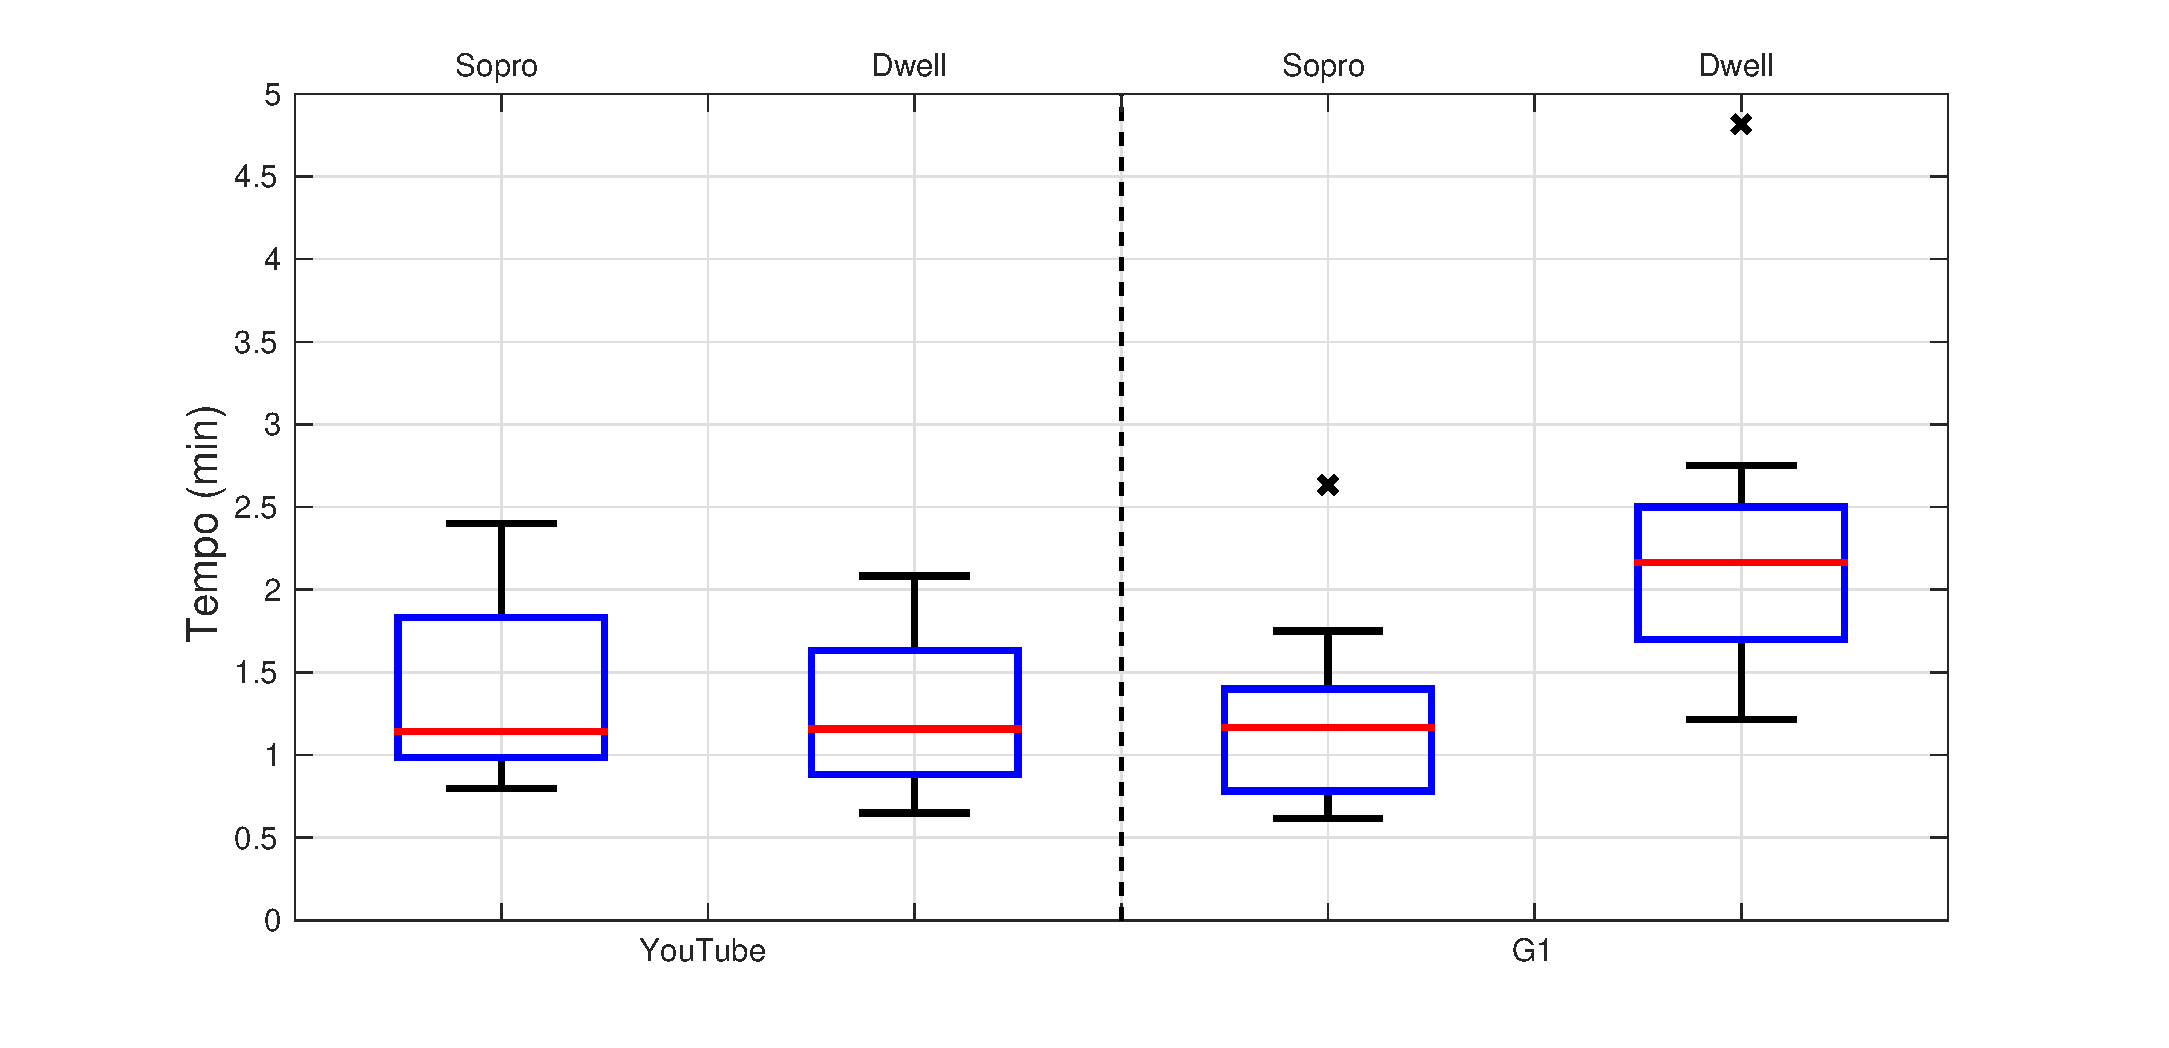
\includegraphics[width=.65\linewidth]{fig/time}
	\vspace{-0.5cm}
	\caption{Distribuição do tempo de conclusão das tarefas.}
	\vspace{-1cm}
	\caption*{\textbf{Fonte: }Elaborada pelo autor.}
	\label{fig:tempo}
\end{figure}

\vspace{-0.5cm}
Analisando a Figura~\ref{fig:tempo}, é possível perceber que, para o YouTube, o
\textit{dwell time} foi o método em que a maioria das pessoas levou menos tempo
para completar a tarefa. Isso pode ser percebido pela amplitude das caixas.
A maioria das pessoas precisou de 50 segundos (50s) a 1 minuto e 40 segundos
(1m40s) para terminar a tarefa do YouTube. Por outro lado, com o dispositivo
baseado em sopro, a maioria das pessoas levou de 1min a 1min50s para concluir a
tarefa.

Já, para o \textit{website} G1, os participantes levaram menos tempo
para finalizar a tarefa utilizando o método de clique baseado em sopro.
A maioria precisou de 45s a 1min30s para terminar a tarefa do G1. Apenas uma
pessoa levou quase 3 minutos para concluir as tarefas do G1, o que explica o
valor de \textit{outlier} exibido como um ``x'' acima da respectiva caixa do
G1. Com o \textit{dwell time}, na tarefa do G1, também houve um caso
\textit{outlier} onde um voluntário completou a tarefa em quase 5 minutos, no
entanto, a maioria dos participantes precisou de 1min45s a 2min30s para terminar
essa tarefa, um tempo superior ao método de clique baseado em sopro.

Como o primeiro método de interação não convencional foi o dispositivo de sopro,
os participantes estavam mais familiarizados quando as tarefas foram executados
pela segunda vez (utilizando o \textit{dwell time}). Isso pode ser observado no
tempo em que os usuários gastaram para executar a tarefa do YouTube, onde o
\textit{dwell time} foi o método alternativo de clique em que  os participantes
levaram menos tempo para concluir a tarefa. No entanto, para o G1, mesmo os
participantes já sabendo exatamente todos os passos da tarefa (pois eles já
tinham executado-a anteriormente com o dispositivo de sopro), o tempo foi maior
com o \textit{dwell time}. Isso aconteceu porque o G1, assim como diversos
outros \textit{websites}, não é adaptado para tecnologias alternativas que usam
o \textit{dwell time} como método de clique, o que dificulta a seleção
correta dos itens desejados no menu, especialmente devido à proximidade entre os
itens, os quais são expandidos apenas passando o ponteiro do mouse sobre eles.

\end{subsection}

\begin{subsection}{Quantidade de Cliques}

\begin{figure}[!b]
	\centering
	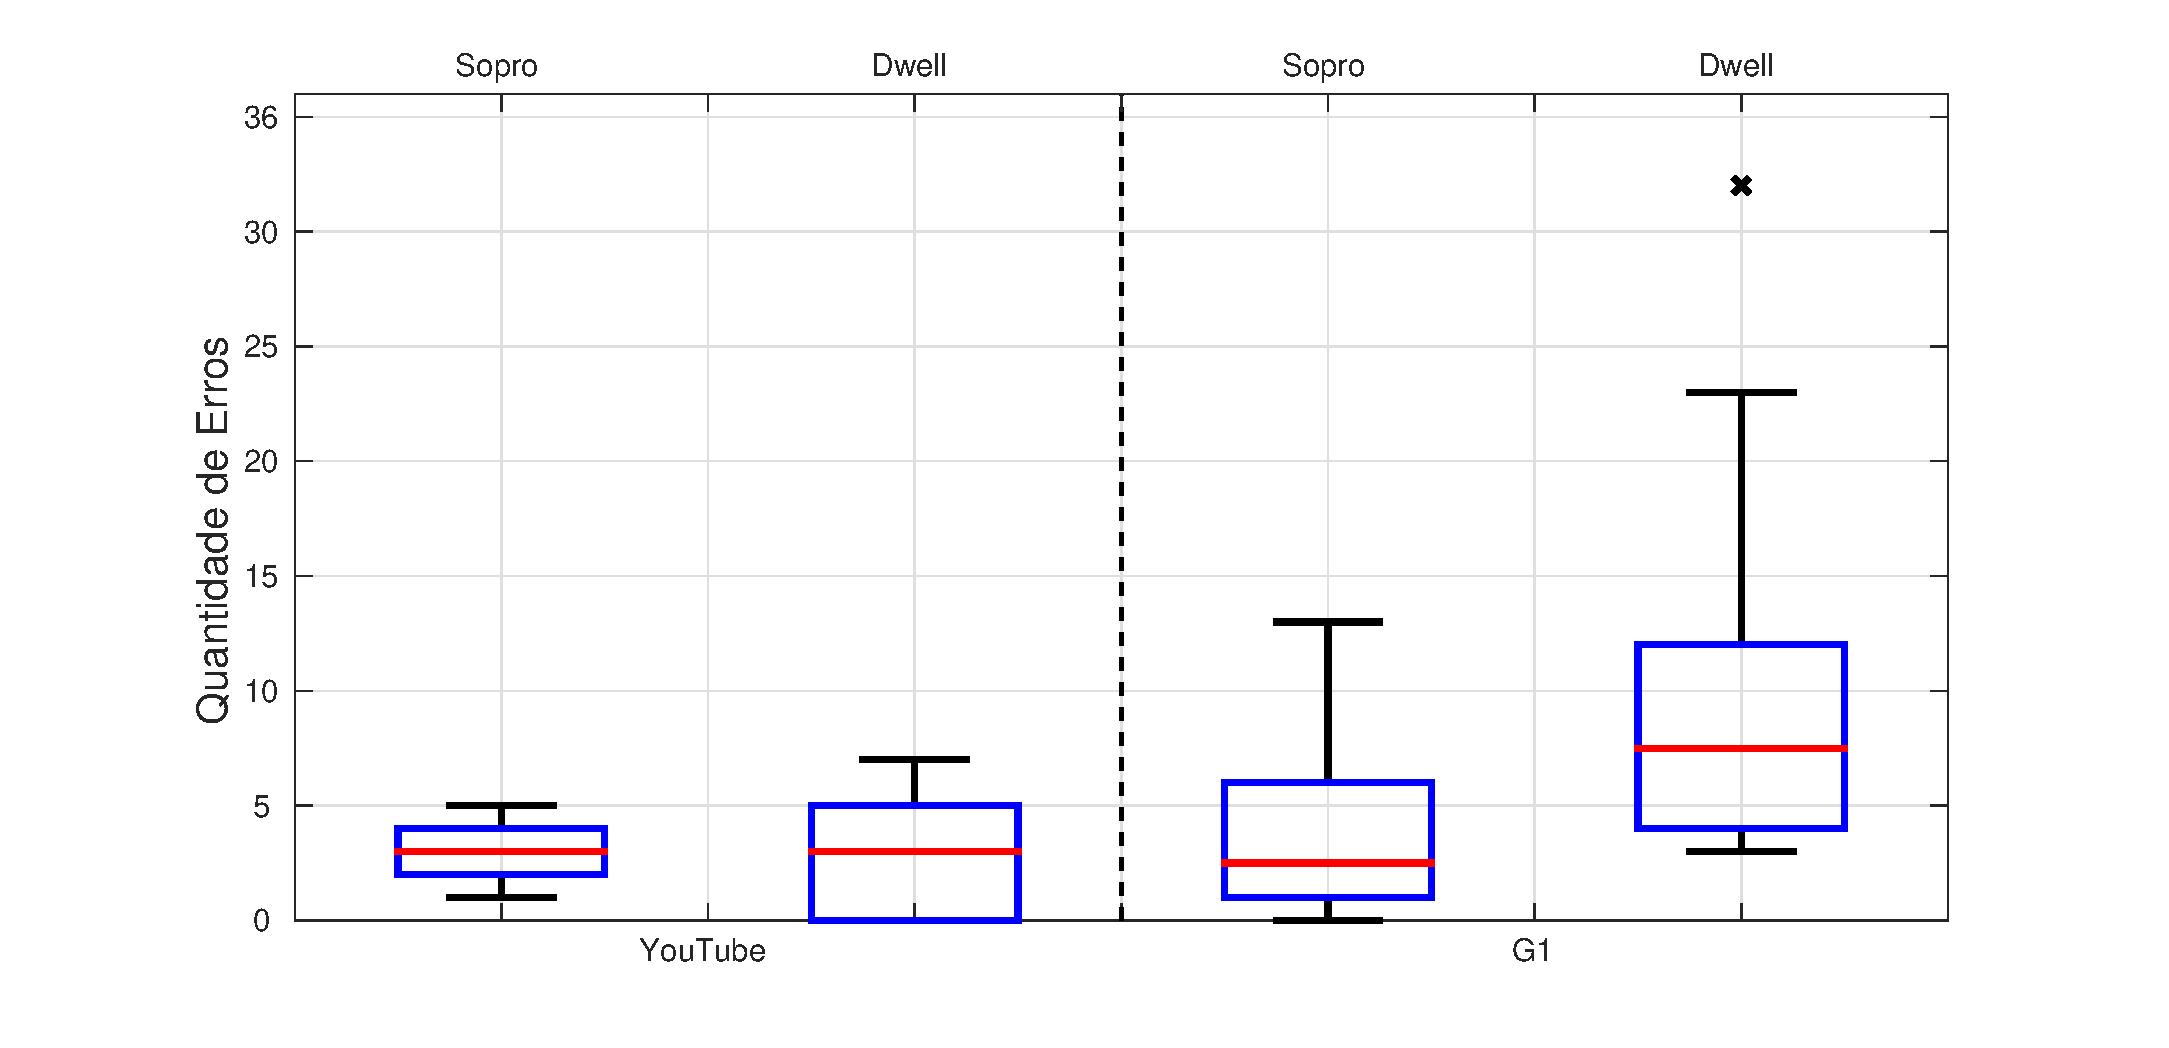
\includegraphics[width=.65\linewidth]{fig/erros}
	\vspace{-0.7cm}
	\caption{Distribuição da quantidade de erros cometidos em cada tarefa.}
	\vspace{-1cm}
	\caption*{\textbf{Fonte: }Elaborada pelo autor.}
	\label{fig:cliques}
\end{figure}
A Figura~\ref{fig:cliques} mostra a quantidade de erros de clique (cliques
involuntários ou sem sucesso), cometidos pelos usuários em cada tarefa. Alguns
participantes realizaram a tarefa do YouTube usuando o \textit{dwell time} sem
erros de cliques, representado pela caixa em azul a partir do zero, fato que não
aconteceu com a ferramenta baseada em sopro. No entanto, na tarefa do G1, o
número de erros aumentou consideravelmente no \textit{dwell time}, onde a
maioria dos voluntários errou entre 4 a 12 vezes.


A maioria dos dos erros de cliques cometidos pelos participantes com o
dispositivo baseado em sopro foi causado por cliques sem sucesso, onde a pessoa
soprava diretamente no transdutor piezoelétrico e o clique não ocorria. Isso
aconteceu principalmente no YouTube, pois essa tarefa foi a primeira a ser
realizada pelos participantes e eles não sabiam ainda exatamente a intensidade
correta de sopro para que o clique ocorresse. Porém, isso não aconteceu com o
\textit{dwell time}, pois a função de clique é ativada depois de um certo
tempo em que o cursor do \textit{mouse} fica sobre uma mesma área. Portanto,
todos os erros cometidos pelos participantes utilizando o \textit{dwell time}
foram causados por cliques involuntários.

As Figuras~\ref{fig:dwellclicks} e~\ref{fig:puffclicks} mostram a quantidade
total de cliques executados pelos usuários utilizando o \textit{dwell time} e o
dispositivo baseado em sopro, respectivamente. A quantidade mínima necessária
para a conclusão das duas tarefas era de seis cliques para a tarefa do YouTube e
quatro cliques para a tarefa do G1. Foram considerados os cliques
realizados corretamente, os cliques involuntários e os
cliques errados (quando o usuário clicava intencionalmente em itens que não
estavam previstos nas tarefas).

É importante ressaltar que eViacam apresentou alguns problemas em detectar a
face do partcipante, e isso afetou diretamente a quantidade de cliques
realizados. A detecção facial falhou diversas vezes quando o participante
tentava posicionar o ponteiro do \textit{mouse} nos cantos da tela. À medida que
o cursor se aproximava dos cantos, a velocidade no movimento do cursor
(controlada pelo rastreador de face do eViacam) diminuía, o que causou muitos
cliques involuntários quando os usuários estavam realizando as tarefas com o
\textit{dwell time}, pois o cursor ficava sobre uma determinada área por tempo
suficiente para que a ação de clique fosse executada.

\begin{figure}[!h]
	\centering
	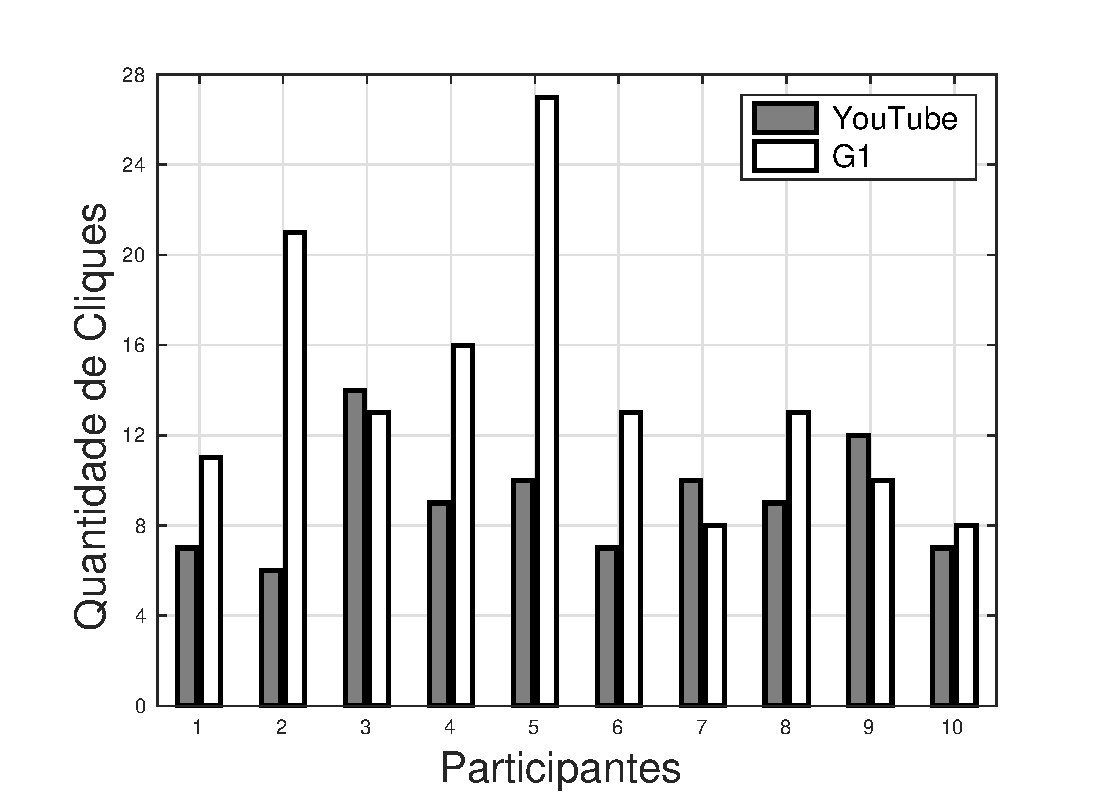
\includegraphics[width=.7\linewidth]{fig/DwellClicks}
	\caption{Quantidade de cliques de cada tarefa, utilizando o \textit{dwell time}.}
	\vspace{-1cm}
	\caption*{\textbf{Fonte: }Elaborada pelo autor.}
	\label{fig:dwellclicks}
\end{figure}

Devido a isso, a quantidade de cliques quando os usuários utilizaram o
\textit{dwell time}, como mostrado na Figura~\ref{fig:dwellclicks}, foi bastante
alta. No total, 90\% dos participantes não conseguiram concluir a tarefa do
YouTube com o valor mínimo de cliques estipulados (seis cliques). A situação
piorou na tarefa o G1, uma vez que nenhum participante conseguiu terminar a
tarefa realizando apenas a quantidade mínima de cliques, resultando em uma média 
bem alta: 14 cliques para uma tarefa que exigia apenas quatro.

~

~
  
A quantidade de cliques foi maior na tarefa do G1 devido à precisão
relativamente alta necessária para selecionar os pontos desejados. O voluntário
tentava clicar em ``economia'', mas acabava clicando no item ``educação'' devido
a grande proximidade desses itens localizados no menu do \textit{website}
(ver Figura~\ref{fig:g1}). Isso ocorreu com diversos participantes, que muitas
vezes ficaram frustrados por não conseguir clicar no item desejado.
\vspace{-0.5cm}
\begin{figure}[!h]
	\centering
	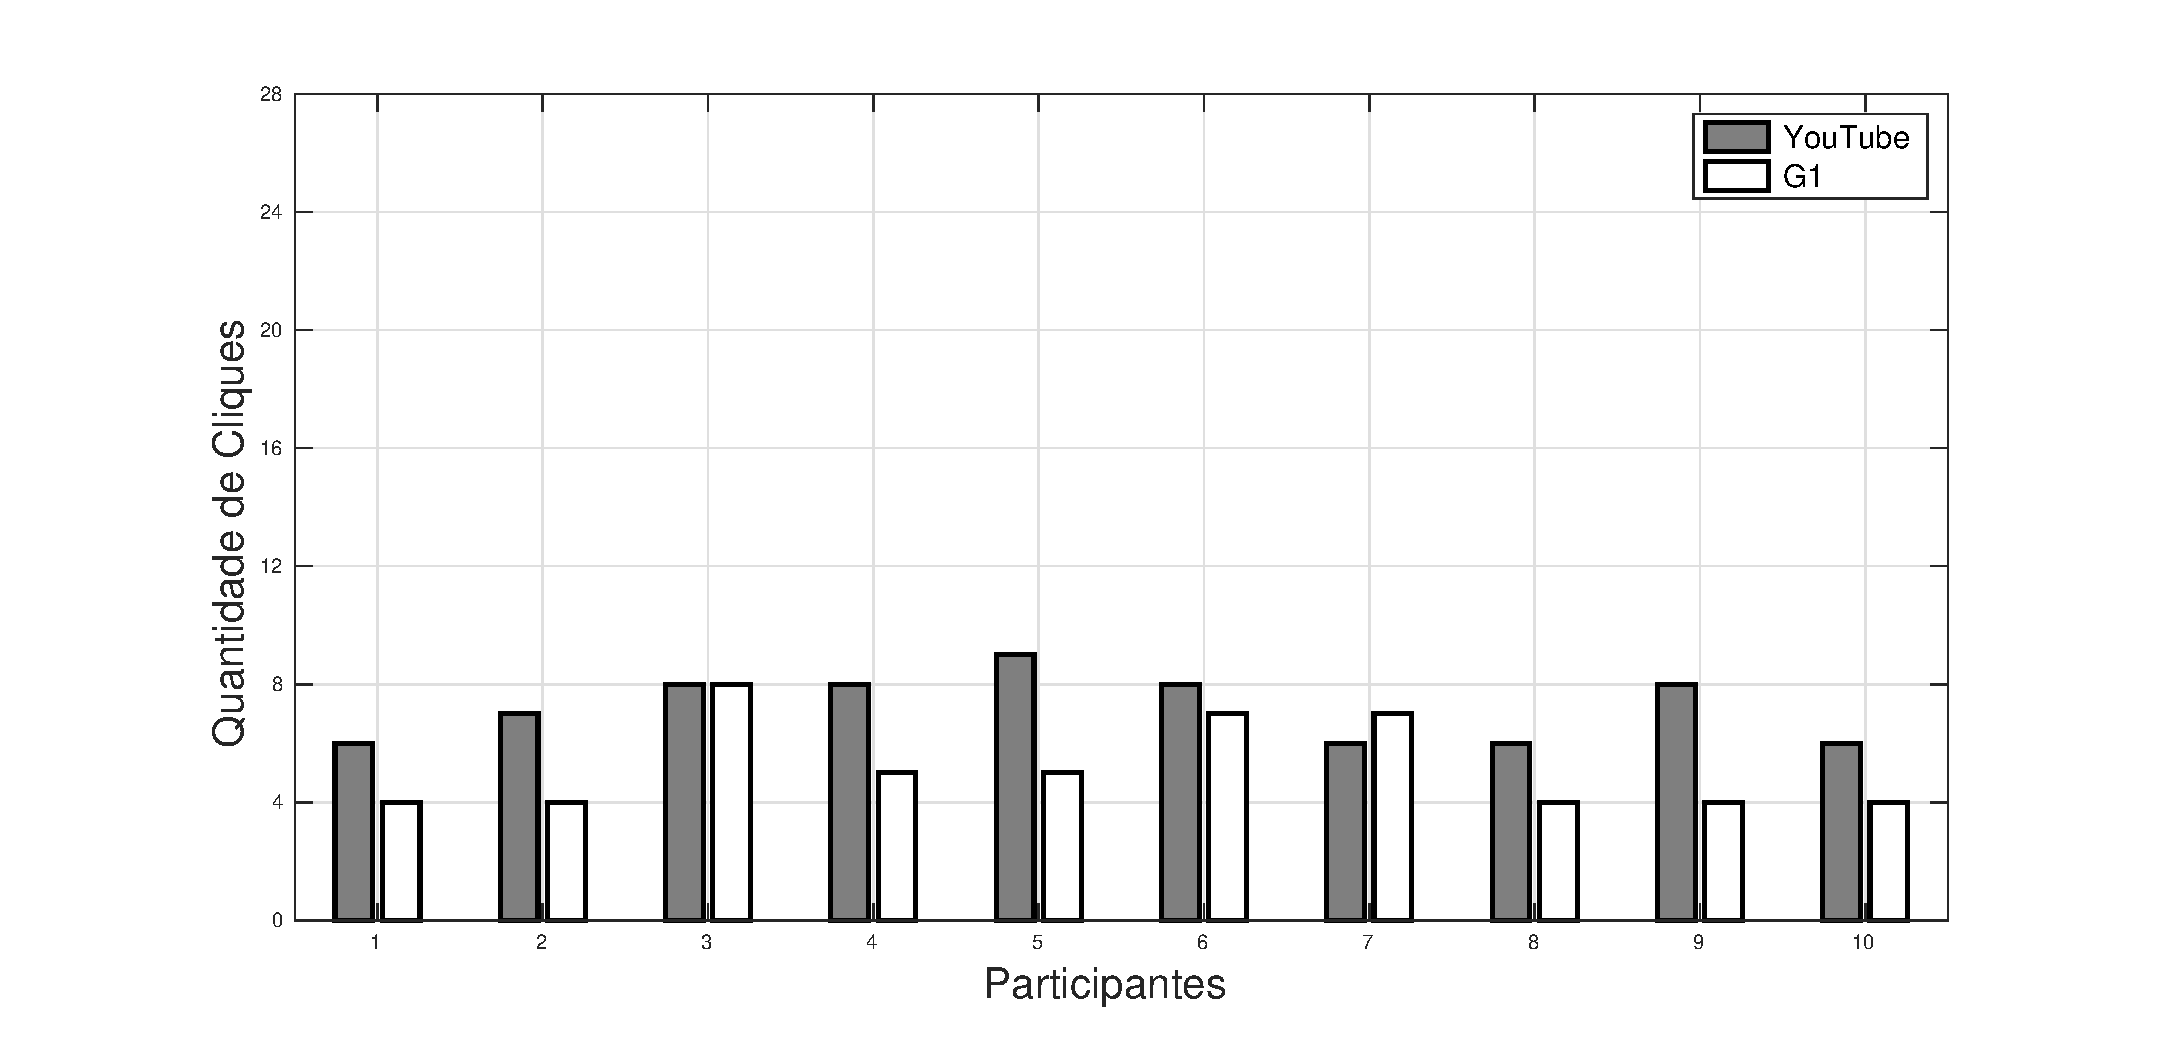
\includegraphics[width=0.7\linewidth]{fig/PuffClicks}
	\caption{Quantidade de cliques de cada tarefa, utilizando o dispositivo baseado em sopro.}
	\vspace{-1cm}
	\caption*{\textbf{Fonte: }Elaborada pelo autor.}
	\label{fig:puffclicks}
\end{figure}

No entanto, com o dispositivo baseado em sopro, os participantes realizaram
menos cliques do que com o \textit{dwell time}, como pode ser visto na
Figura~\ref{fig:puffclicks}. Na tarefa do YouTube, por exemplo, quatro pessoas
(os participantes 1, 7, 8 e 10) conseguiram concluir a tarefa utilizando somente
seis cliques. No G1, 50\% das pessoas completaram a tarefa utilizando o número
mínimo de cliques necessários, enquanto que os demais precisaram de oito clique
no máximo.

À primeira vista, quando os participantes utilizaram o protótipo baseado em
sopro, o maior número de cliques ocorreu na tarefa do YouTube. Isso de fato
aconteceu, mas devido ao eViacam, que muitas vezes falhava em detectar o rosto
do participante durante a tentativa de posicionar o cursor nos cantos inferiores
do monitor, como relatado anteriormente.
  
Na tarefa do G1, por outro lado, a dificuldade foi novamente devido às áreas
clicáveis do menu desse \textit{website} estarem muito próximas umas das
outras. No entanto, notou-se que algumas pessoas moviam levemente a cabeça
enquanto sopravam, principalmente devido à força aplicada no peito durante a
expiração do ar. Consequentemente, o cursor do \textit{mouse} também se movia e
esse movimento era suficiente para que o ponteiro se deslocasse para outra
região, fazendo o usuário clicar em um alvo indesejado.
\end{subsection}

\begin{subsection}{Questões de Múltipla Escolha}
A seguir, os resultados das seis questões de múltipla escolha respondidas pelos
voluntários são mostrados. Essas questões podem ser visualizadas na
Tabela~\ref{tab:quest}.

\begin{table}[!h]
\centering
\small
\def\arraystretch{1.0}
\begin{tabular}{c|ll}
	\hline
	\hline
	 \textbf{Pergunta} &\multicolumn{2}{c}{\textbf{Resposta}} \\
	\hline
	 Como foi sua experiência usando esse método alternativo de clique? & 1 -- insuficiente        & 5 -- excelente   \\
	 O que você achou do tempo para realizar a tarefa?                  & 1 -- lento               & 5 -- rápido      \\
	 Como foi a precisão para realizar a tarefa?                        & 1 -- insuficiente        & 5 -- excelente   \\
	 Como foi o esforço cognitivo para realizar a tarefa?               & 1 -- alto                & 5 -- baixo       \\
	 Como foi o esforço físico para realizar a tarefa?                  & 1 -- alto                & 5 -- baixo       \\
	 Você se concentrou mais na tarefa ou no método de clique?          & 1 -- no método           & 5 -- na tarefa   \\
	%\hline
	%\textbf{\#}& \multicolumn{3}{c}{Based on your experience, what suggestions
	%would you give about the puff-based device?} \\
	\hline
	\hline
\end{tabular}
\caption{Perguntas utilizadas no questionário objetivo.}
\label{tab:quest}
\end{table}

As Figuras~\ref{fig:DwellQuestions} e~\ref{fig:PuffQuestions} mostram uma visão
geral de todas as respostas do questionário de múltipla escolha dadas pelos
participantes. A escala Likert foi utilizada para representar as respostas, que
variam de 1 a 5, para ambos os métodos de clique utilizados no teste.

A resposta 1, colorida em vermelho, significa muito ruim,
enquanto a resposta 5, colorida em verde escuro, significa muito bom. Ao
realizar um rápida comparação entre as respostas, é possível afirmar que os
participantes se sentiram mais satisfeitos com o desempenho geral do dispositivo
de sopro do que com o \textit{dwell time}, pois a maioria das respostas
para o método de clique baseado em sopro, tanto para tarefa do YouTube quanto
para o G1, realizadas foram 4
ou 5, como mostrado na Figura~\ref{fig:PuffQuestions}. Por outro lado, as 
respostas para o \textit{dwell time} variaram de 3 a 5, conforme mostrado na
Figura~\ref{fig:DwellQuestions}.  

\begin{figure}[!h]
	\centering
	\begin{minipage}[c]{\textwidth}
	\centering
	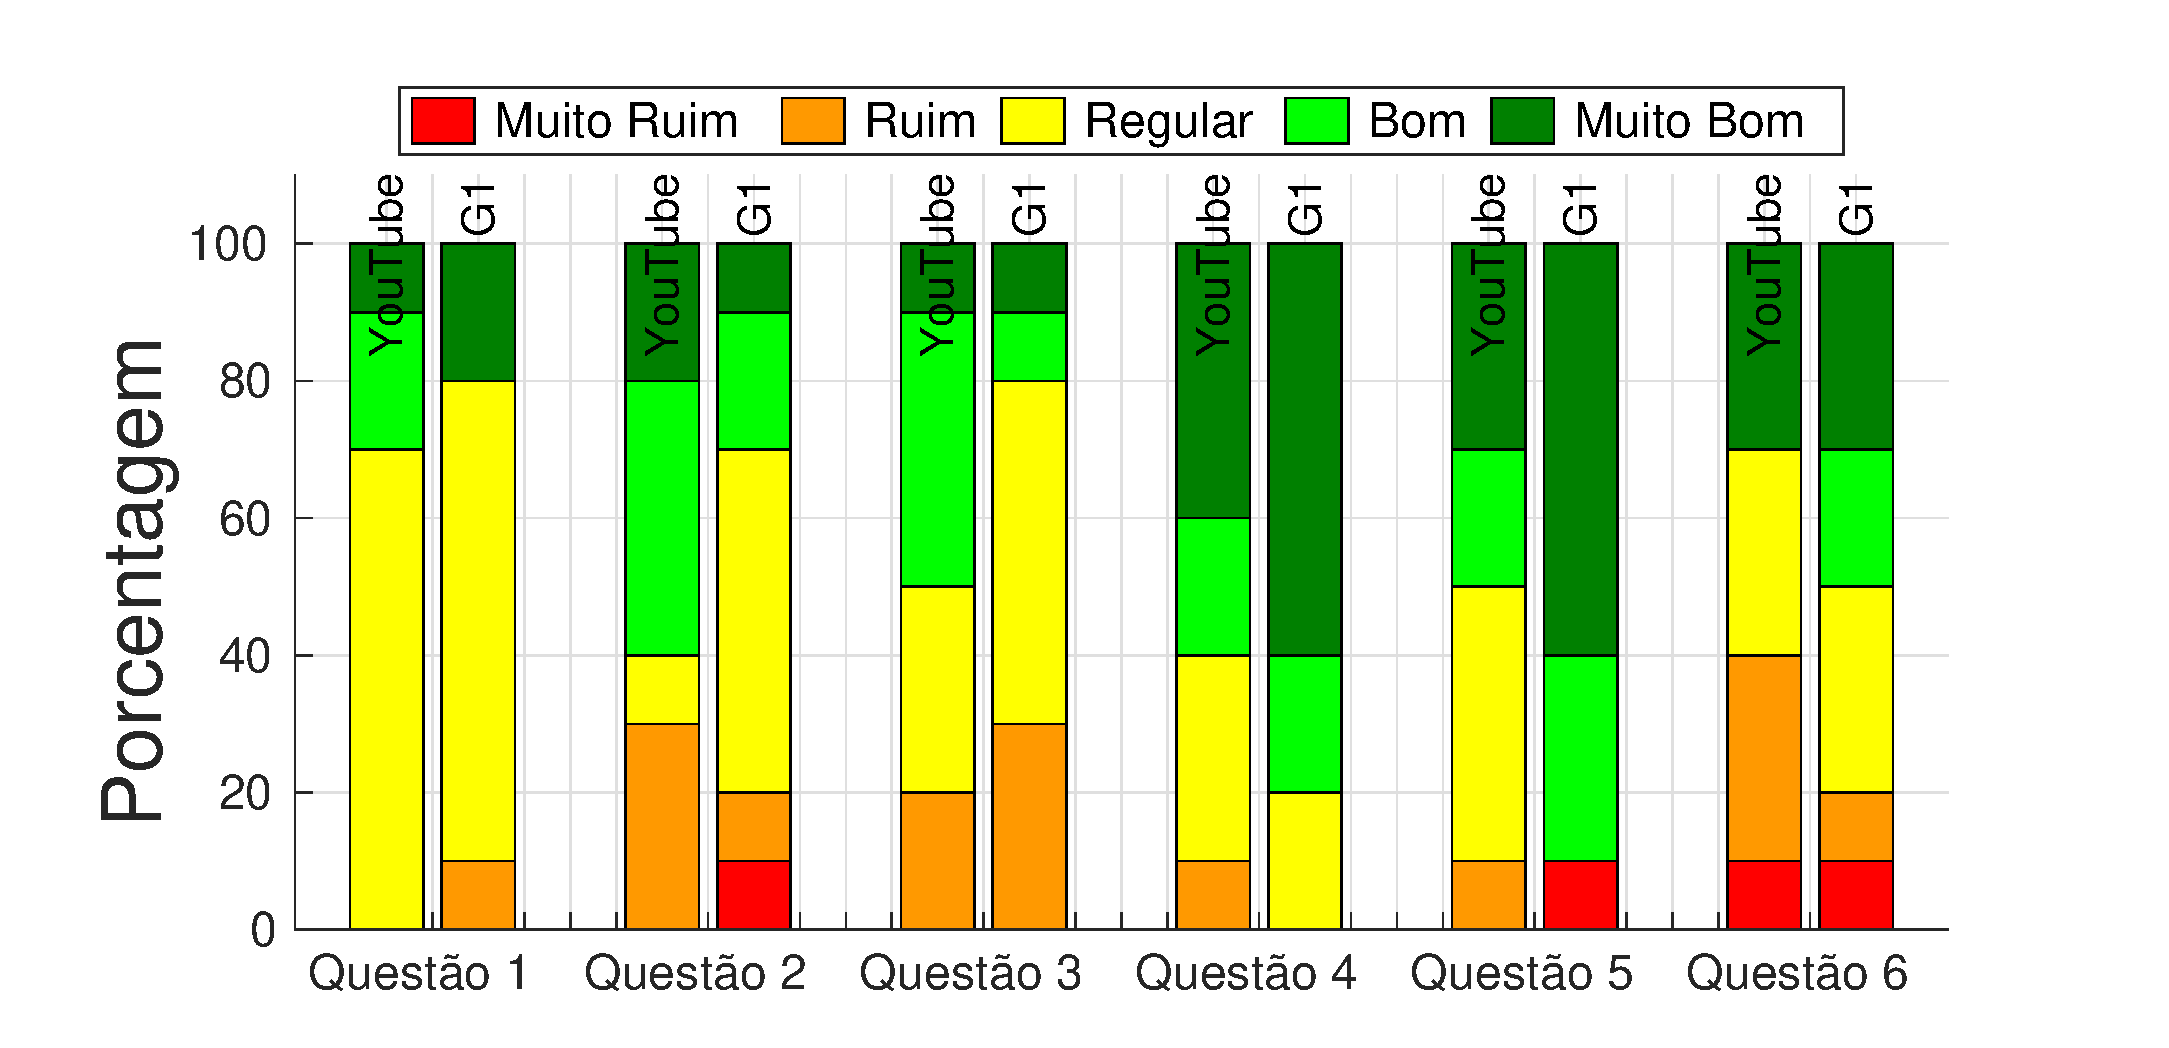
\includegraphics[width=0.95\linewidth]{fig/DwellQuestions}
	\vspace{-0.5cm}
	\caption{Escala Likert das respostas do \textit{dwell time}.} 
	\vspace{-1cm}
	\caption*{\textbf{Fonte: }Elaborada pelo autor.}
	\label{fig:DwellQuestions}
	\end{minipage}
\end{figure}

\begin{figure}[!h]
	\centering
	\begin{minipage}[c]{\textwidth}
	\centering
	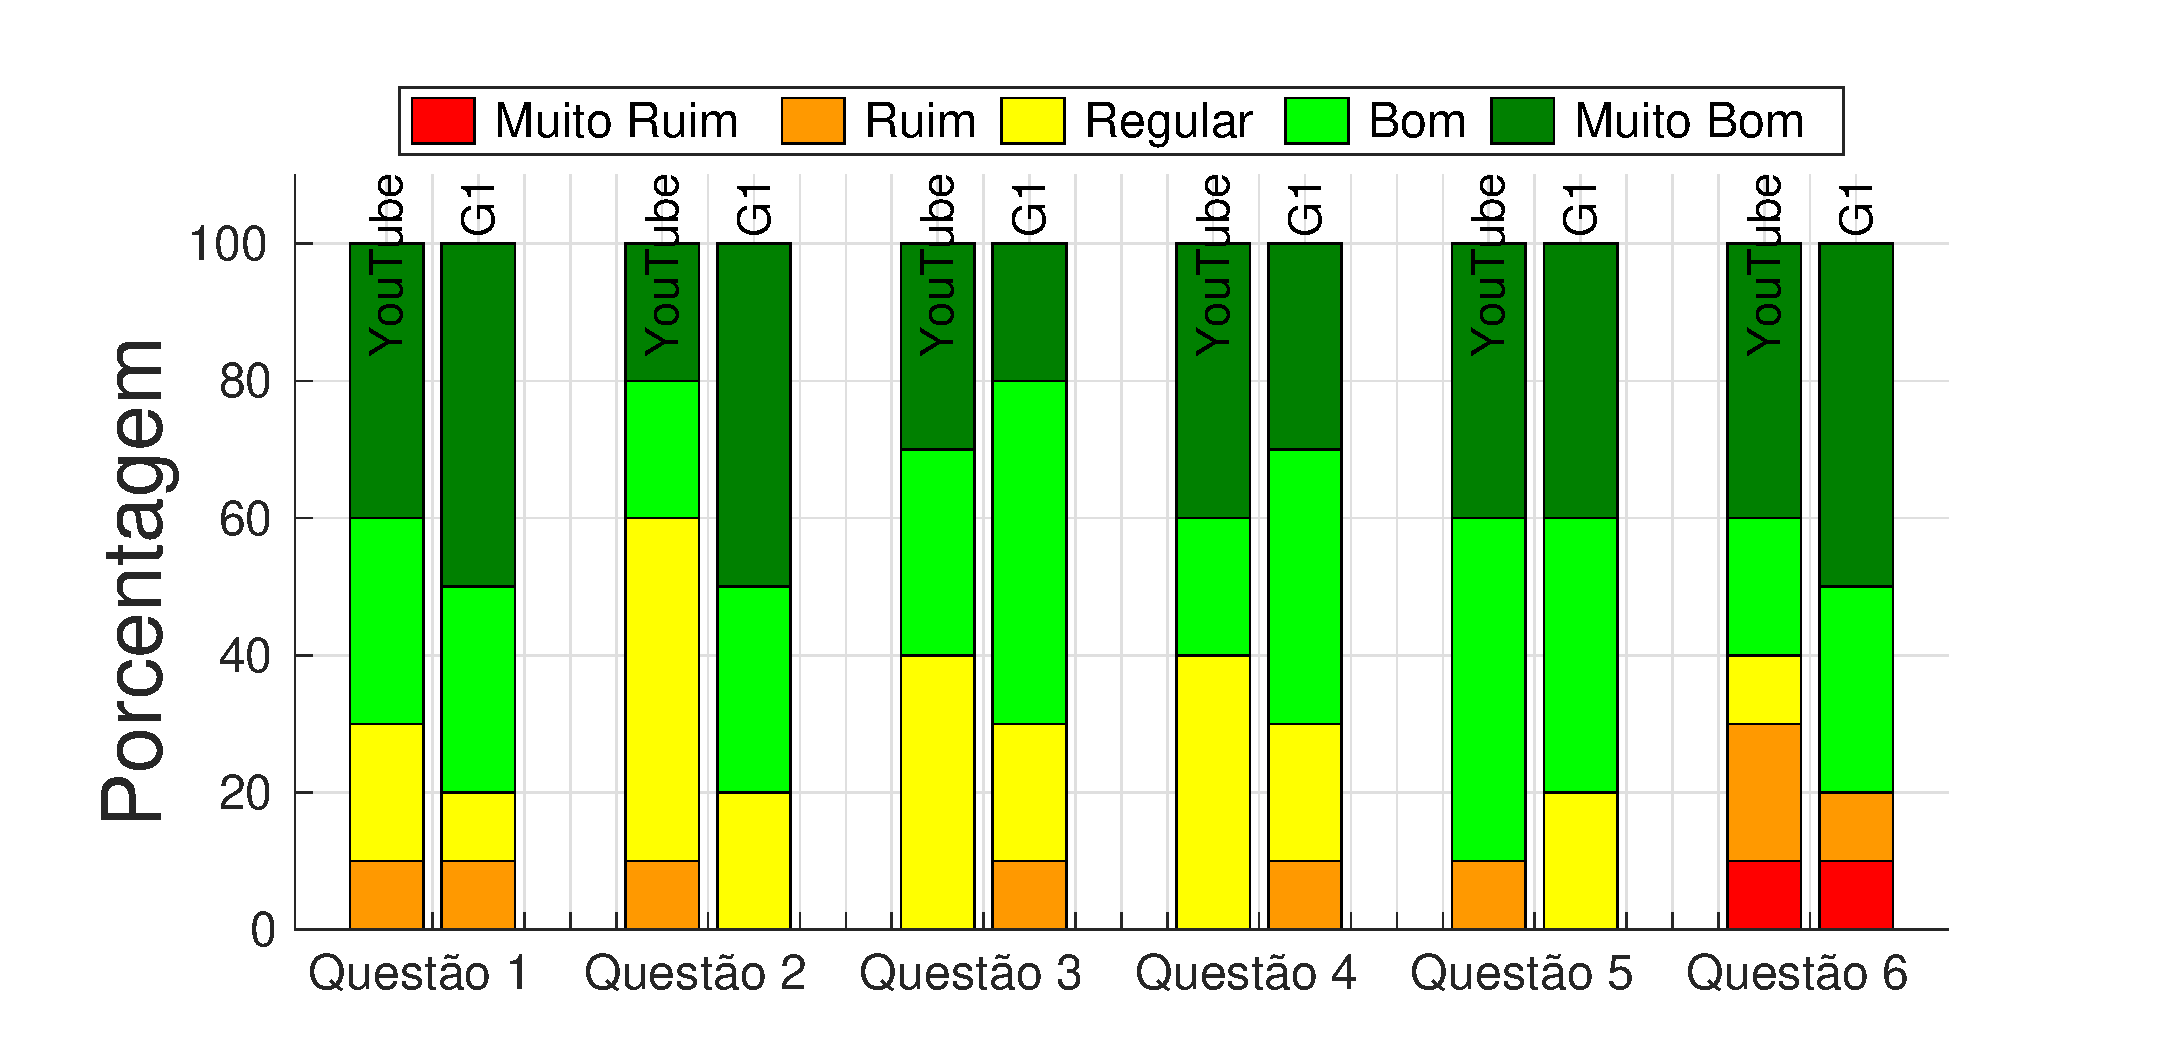
\includegraphics[width=0.95\linewidth]{fig/PuffQuestions}
	\vspace{-0.5cm}
	\caption{Escala Likert das respostas do protótipo baseado em sopro.}
	\vspace{-1cm}
	\caption*{\textbf{Fonte: }Elaborada pelo autor.}
	\label{fig:PuffQuestions}
	\end{minipage}
\end{figure}



É notório a quantidade superior de respostas que variaram de 1 a 3 para o
\textit{dwell time} em comparação com o clique baseado em sopro. Isso significa
que a maioria das pessoas não ficaram tão satisfeitas com o desempenho do
\textit{dwell time}. De acordo com os participantes, essa insatisfação ocorreu
principalmente devido à tarefa do G1 ser considerada mais problemática de ser
realizada utilizando o \textit{dwell time}, pois eles precisaram mover o
cursor do \textit{mouse} mais lento que o normal devido à proximidade dos itens
clicáveis localizados no menu do \textit{website}. Diversas vezes, a lentidão do
ponteiro do \textit{mouse} provocou cliques involuntários devido o cursor ficar
sobre uma determinada área por tempo suficiente para a ocorrer a ativação do
clique.

Na questão 1, os usuários relataram que a exeperiência de uso, com o
\textit{dwell time}, foi regular, como pode ser percebido pela maior
concentração de retângulos em amarelo para ambas as tarefas realizadas. Por
outro, com o dispositivo baseado em sopro, a experiência de uso foi considerada
boa, visto que mais de 60\% dos participantes responderam 4 ou 5.  Quanto ao
tempo gasto para realizar uma tarefa, perguntado na questão 2, analisando apenas
a tarefa do G1, novamente os usuários apontaram que o clique realizado com o
dispositivo baseado em sopro foi melhor, uma vez que apenas 30\% dos
participantes deu uma resposta abaixo de 3, um fato que não ocorreu para o
clique realizado com o \textit{dwell time}.

Os participantes também não ficaram satisfeitos com a precisão do \textit{dwell
time}, já que apenas 20\% dos voluntários deu nota 4 ou 5 para a pergunta 3 na
tarefa do G1. No YouTube, os participantes não tiveram dificuldade em realizar a
tarefa, visto que não era necessário uma grande precisão para executá-la. 

O esforço cognitivo, perguntado na questão 3, foi muito similar para ambos os
métodos de clique. Contudo, analisando a questão 4, onde se perguntava sobre o
esforço físico para realizar as tarefas, é possível notar que na tarefa do
YouTube, o dispositivo baseado em sopro provocou menos esforço físico nos
participantes, pois 90\% das respostas foram 4 ou 5 enquanto que apenas 50\%
das repostas foram 4 ou 5 para o \textit{dwell time}. Por outro lado, na tarefa
do G1, o \textit{dwell time} foi o método que necessitou menos esforço físico
para realizar a tarefa, pois 60\% das respostas foi 5 e outros 30\% das
respostas foi 4. Essa quantidade foi maior que as repostas para o método de
clique baseado em sopro, onde 40\% dos usuários respondeu 5 e outros 40\%
respondeu 4.

A razão pela qual o método de clique baseado em sopro exigiu mais esforço físico
para realizar a tarefa do G1 pode ser a dificuldade que os voluntários tiveram
em realizar a ação de sopro sem movimentar muito a cabeça. Como os itens do menu
do G1 são bastantes próximos uns dos outros, alguns movimentos (incluindo os
executados durante a inspiração e expiração pela boca ao executar a ação de
sopro, que afeta praticamente todo o torso humano), deslocavam o ponteiro do
alvo desejado.

Por fim, é possível observar na última questão que os participantes se sentiram
mais à vontade ao utilizar o dispositivo baseado em sopro, pois a maioria
respondeu 4 ou 5, o que significa que os voluntários se concentraram mais na
realização da tarefa do que no método de clique. Esse fato não se confirmou com o
\textit{dwell time}, pois a maioria das respostas variou de 1 a 3, ou seja, esse
método de clique interferiu na concentração dos participantes na realização das
tarefas. 

\end{subsection}

\begin{subsection}{Discussão Sobre a Questão Subjetiva}

No final dos testes, cada participante foi convidado a responder em um
formulário virtual a seguinte pergunta: ``Com base na sua experiência de uso,
que sugestões você daria para melhoria do dispositivo baseado em sopro?''. Eles 
foram instruídos a se sentir completamente livres para escrever críticas e 
apontar sugestões para a melhoria do dispositivo proposto. Todas as respostas
foram lidas e serão sintetizadas a seguir.

%O maior problema identificado pela maioria dos participantes foi uso do
%\textit{software} eViacam. A falha no rasteamento da face do usuário ao
%posicionar o cursor do \textit{mouse} nos cantos da tela e em ícones pequenos
%frustrou bastante os participantes, que sugeriram a troca do \textit{software}
%de controle do ponteiro do \textit{mouse}.

O dispositivo baseado em sopro proposto neste trabalho foi considerado uma boa
ferramenta para ser utilizada como um método alternativo de clique. Apesar do
bom desempenho do protótipo desenvolvido, ocorreram alguns problemas encontrados
pelos participantes, principalmente no que diz respeito a cliques involuntários.
Os voluntários sugeriram a substituição do \textit{headset} utilizado como
suporte de sustentação do acionador externo desenvolvido, pois ocorreram alguns
choques mecânicos causados por essa ferramenta quando os participantes moviam
a cabeça muito rápido.

Houve também alguns casos onde o participante realizou a ação de sopro e o
clique não ocorreu. Isso aconteceu devido à intensidade do sopro não ser
suficiente para a ativação do clique. Para a maioria dos participantes, a
sensibilidade do dispositivo baseado em sopro estava adequada, pois era
necessário um sopro relativamente fraco para a ativação do clique. No entanto,
alguns voluntários relataram que se sentiriam mais confortáveis se a
sensibilidade fosse aumentada. %Há um potenciômetro acoplado no dispositivo
%proposto que permite o ajuste da sensibilidade, porém apesar de estar ajustado
%em um valor que não necessitava um sopro muito forte nem muito fraco, essa
%sensibilidade gerou desconforto entre alguns usuários. A sugestão dada pelos
%participantes foi a disponibilidade de três níveis de ajuste da sensibilidade
%para que cada usuário possa escolher a intensidade de sopro ideal. 
Eles também enfatizaram que o  dispositivo poderia ter um \textit{feedback}
visual a fim de mostrar para o usuário qual o nível de sensibilidade está
definido no momento.


\end{subsection}

\end{section}

\end{chapter}
